\chapter{Introducción}
\label{cap:introduccion}

% Estilo de párrafo de los capítulos
\setlength{\parskip}{0.75em}
\renewcommand{\baselinestretch}{1.25}
% Interlineado simple
\spacing{1}
% Numeración contenido
\pagenumbering{arabic}
\setcounter{page}{1}

La presente sección tiene como objetivo realizar una contextualización sociocultural del proyecto \textit{VSCode4Teaching} y una cronología de la evolución del proyecto y sus iteraciones previas y, a continuación, exponer la motivación del presente Trabajo Fin de Grado y la necesidad que pretende resolver. Para concluir, se introduce brevemente el formato del presente documento y su división en epígrafes.

\section{Contexto sociocultural}
\label{sec:contxtSocial}
La \textit{Declaración Universal de los Derechos Humanos} aprobada por la Asamblea General de la Organización de las Naciones Unidas en diciembre de 1948 recoge en su artículo 26 que ``toda persona tiene derecho a la educación'', que ``la instrucción elemental es obligatoria'' y que ``la educación tendrá por objeto el pleno desarrollo de la personalidad humana y el fortalecimiento del respeto a los derechos humanos y a las libertades fundamentales'' \cite{ONUDUDH}. Esta declaración continúa vigente y en plena expansión a nivel global, tal como demuestran los \textit{Objetivos de Desarrollo Sostenible} contenidos en la \textit{Agenda 2030} \cite{ONU2030}, un manifiesto de intenciones divulgado por Naciones Unidas en el año 2015 para el desarrollo integral del planeta y sus habitantes. Entre estos objetivos, el cuarto establece la necesidad de ``garantizar una educación inclusiva, equitativa y de calidad'', destacando en su punto B la importancia del avance en los ``programas técnicos, científicos, de ingeniería y de tecnología de la información y de las comunicaciones en los países desarrollados y otros países en desarrollo''.

Cabe conjugar este relevante papel de la educación como valor fundamental para el crecimiento y el desarrollo de la sociedad a nivel global con la incipiente relevancia que la informática tiene en la actualidad: todos los sectores sociales, culturales o laborales se han visto impregnados en mayor o menor medida de las capacidades que la digitalización puede brindarles para alcanzar nuevas cotas de desarrollo. El \textit{Informe sobre la Conectividad Global} elaborado por la Unión Internacional de Telecomunicaciones \cite{UITConectividad}, que es una agencia especializada de Naciones Unidas para las tecnologías de la información y las comunicaciones, refleja que el 63\% de la población global disponía de acceso a Internet en el año 2021, cifra que se reduce significativamente al explorar años anteriores: un 18\% en 2006, un 38\% en 2014 y un 46\% en 2017. Este crecimiento ha venido auspiciado en gran medida por la llegada de las tecnologías a las sociedades menos desarrolladas. Sin embargo, sigue existiendo una brecha en el acceso a Internet: mientras que el 87\% de los habitantes de Europa disfrutan de la red global descentralizada, solo un 33\% de los ciudadanos africanos la emplean. Además, de los habitantes europeos, el 94\% dispone de un acceso con una velocidad igual o superior a 10 Mbps\footnote{Mbps. Abreviatura de ``megabits por segundo''. Por ejemplo, una conexión de 1 Mbps permitirá recibir un máximo de 1000000 bits de información por segundo.}, mientras que en África este porcentaje se reduce hasta el 41\%, mientras que un 46\% disponen de un acceso de entre 2 y 10 Mbps, siendo el 12\% restante conexiones de peor velocidad.

Poniendo el foco en España, la digitalización de la educación es una de las grandes prioridades del marco educativo actual. Así lo refleja la actual Ley Orgánica para la Mejora de la Ley Orgánica de Educación \cite{LOMLOE} (LOMLOE), que trata en su preámbulo la ``necesidad de tener en cuenta el cambio digital que se está produciendo y que afecta a la actividad educativa'', considerando que ``el mundo digital es un nuevo hábitat en el que la infancia y la juventud viven cada vez más'' y que, en consecuencia, ``el sistema eduativo debe adoptar el lugar que le corresponde en el cambio digital, con autención al desarrollo de la competencia digital de los estudiantes de todas las etapas educativas''. Tal es así que, ya en el año 2001, el escritor estadounidense Marc Prensky acuñó el término ``nativos digitales'' para aludir al conjunto de personas que han nacido durante la gran revolución tecnología que ha vivido la sociedad en las últimas décadas \cite{Prensky}.

La educación de los ``nativos digitales'' debe producirse, por tanto, en consonancia con la sociedad en que se desarrollarán sus vidas, en la que deberán desenvolverse con soltura en la utilización de las herramientas informáticas que acompañen sus ámbitos sociocultural y laboral, lo que convierte a la informática en uno de los ejes fundamentales de la educación de los más pequeños de la sociedad. Intrínsecamente, este hecho conduce a la necesidad de la educación en la competencia digital, que toma un papel esencial en todos los currículos educativos de las enseñanzas obligatorias de las distintas comunidades autónomas españolas. Sirva como ejemplo Madrid, en cuyo currículo de enseñanzas para la Educación Secundaria Obligatoria incluye la palabra ``digital'' en 161 de las 321 páginas que lo componen y que establece la presencia de varias asignaturas relacionadas con este ámbito, tales como Tecnología y Digitalización, que es obligatoria en dos cursos de esta etapa educativa; y Ciencias de la Computación, una materia optativa ofrecida posteriormente que busca divulgar el pensamiento computacional, reflejando la vinculación esencial de la digitalización con la educación \cite{CAMCurriculoESO}. Esta educación orientada a la informática requiere que sus docentes dispongan de la capacidad y conocimientos adecuados para poder divulgarlos, por lo que se están ejecutando numerosos programas para la mejora de la competencia digital educativa, como \textit{\#CompDigEdu} \cite{CompDigEduINTEF}, que es un plan de mejora articulado por el Instituto de las Tecnologías Educativas y de Formación del Profesorado (INTEF) que dispone el impulso de la competencia digital mediante la formación a los docentes y el diseño de planes para la expansión tecnológica en los centros educativos.

Este contexto de informatización de la educación y de situación de la competencia digital como un pilar esencial para el desarrollo de la sociedad en el que herramientas como \textit{VSCode4Teaching} toman un papel crucial. Este proyecto busca facilitar la docencia de la computación a través de una aplicación que permite a los dos actores esenciales de la educación, docentes y estudiantes, interactuar en tiempo real a través de una aplicación informática que organiza y facilita las clases en torno a la programación informática.

\section{\textit{VSCode4Teaching}: definición y cronología}
\label{sec:cronologiaProyecto}
\textit{VSCode4Teaching} es una herramienta que permite a docentes y estudiantes interactuar durante la enseñanza de la programación informática, facilitando su impartición y organización. Para ello, permite a los docentes crear cursos que, a su vez, quedan compuestos por ejercicios que están dotados de una plantilla inicial. Los estudiantes, por su parte, pueden visualizar los ejercicios de los cursos en los que estén matriculados y realizarlos, para lo que tendrán como punto de partida la plantilla propuesta por sus profesores y sobre la que realizarán modificaciones que se irán guardando progresivamente y quedando a disposición de los docentes. Una vez finalizados los ejercicios, los estudiantes los marcan como completados, bloqueando así la posibilidad de realizar nuevas ediciones. Los docentes disponen de información actualizada en tiempo real acerca del progreso de los estudiantes en la realización de los ejercicios y pudiendo visualizar los ficheros de cada propuesta de resolución en el momento que lo deseen.

El proyecto \textit{VSCode4Teaching} se remonta al curso académico 2019-20, cuando Iván Chicano Capelo lo inició en el contexto de su Trabajo Fin de Grado \cite{TFG_Ivan}. Este trabajo sentó las bases del proyecto y dio lugar a una aplicación compuesta por dos componentes organizados en una arquitectura cliente-servidor. El cliente es una extensión para Visual Studio Code\footnote{Visual Studio Code. Entorno de desarrollo integrado divulgado como \textit{software} libre popularizado por su sencillez y gratuidad (más información en la \referenciaSeccion{subsec:herIDEs}).} que permite a docentes y estudiantes interactuar desde su entorno de desarrollo con el servidor, proporcionando una interfaz que usuario para consultar sus cursos impartidos o matriculados, los ejercicios de los que se componen y el estado de progreso en la realización de cada uno de ellos, permitiéndoles descargar sus ficheros asociados y visualizarlos dentro del propio entorno de desarrollo. Por otro lado, el servidor es el responsable de, a través de una API\footnote{API. Siglas de ``interfaz de programación de aplicaciones'' (del inglés \textit{Application Programming Interface}). Es un componente \textit{software} que permite la comunicación de agentes externos con el sistema que lo incorpora.}, la interacción de la extensión con los sistemas de persistencia, ya que se ocupa de almacenar todas los ficheros de las propuestas de resolución de ejercicios y, además, todos los datos de la aplicación en una base de datos.

Tras este \textbf{primer} paso en el proceso evolutivo del proyecto, la aplicación ya disponía de los dos roles de usuarios ---estudiantes y profesores--- y de múltiples procesos de negocio implementados. Los docentes ya disponían de capacidades para: crear, actualizar y eliminar cursos, matricular y desmatricular estudiantes en sus cursos, añadir nuevos ejercicios cargando su plantilla asociada, modificar y eliminar los ejercicios, consultar en un \textit{dashboard} información sobre su realización por parte de los estudiantes y obtener bajo demanda sus ficheros ---tal como muestra la \referenciaFigura{fig:historiaProyecto1Dashboard}---, compartir un código para la automatriculación de estudiantes en los cursos, facilitar la comparación de las propuestas del estudiantado con la plantilla original de forma gráfica ---reflejada en la \referenciaFigura{fig:historiaProyecto1Comparacion}--- e introducir comentarios en las líneas de los ficheros de las propuestas de los estudiantes.

Los estudiantes, por otro lado, pueden: registrarse libremente en la aplicación, visualizar sus cursos matriculados, inscribirse en cursos nuevos a partir de un código de compartición, acceder a los ejercicios que componen los cursos y descargar los ficheros en su último estado de modificación (siendo este la plantilla inicial en caso de no haberlos iniciado), modificar y guardar su progreso en la realización de los ejercicios ---sincronizándose con el servidor--- y marcar los ejercicios como finalizados, impidiéndose la sincronización de sucesivas ediciones.

\begin{figure}[ht!]
    \centering
    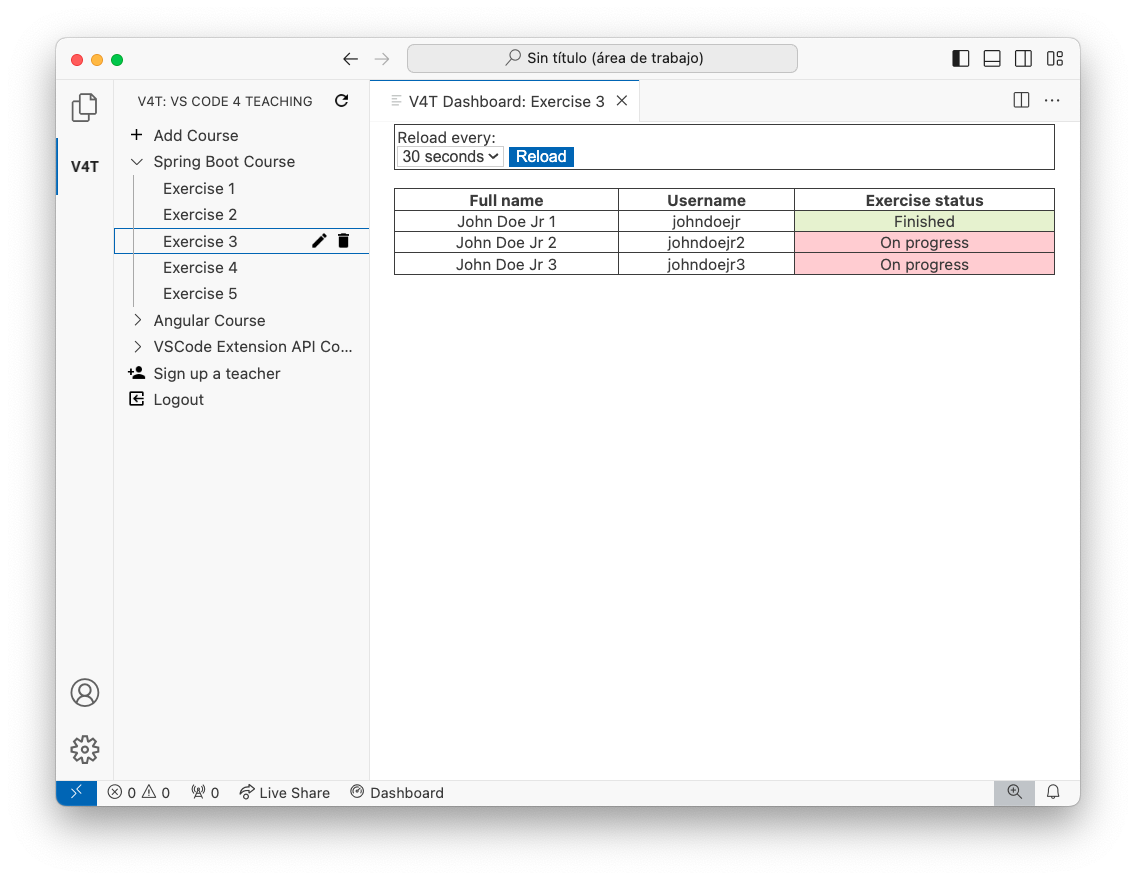
\includegraphics[width=0.825\linewidth]{imagenes/utilizadas/1-introduccion/historia-tfg1-dashboard.png}
    \caption{Captura del \textit{dashboard} para el seguimiento del progreso de los ejercicios en el primer TFG.}
    \label{fig:historiaProyecto1Dashboard}
\end{figure}

\begin{figure}[ht!]
    \centering
    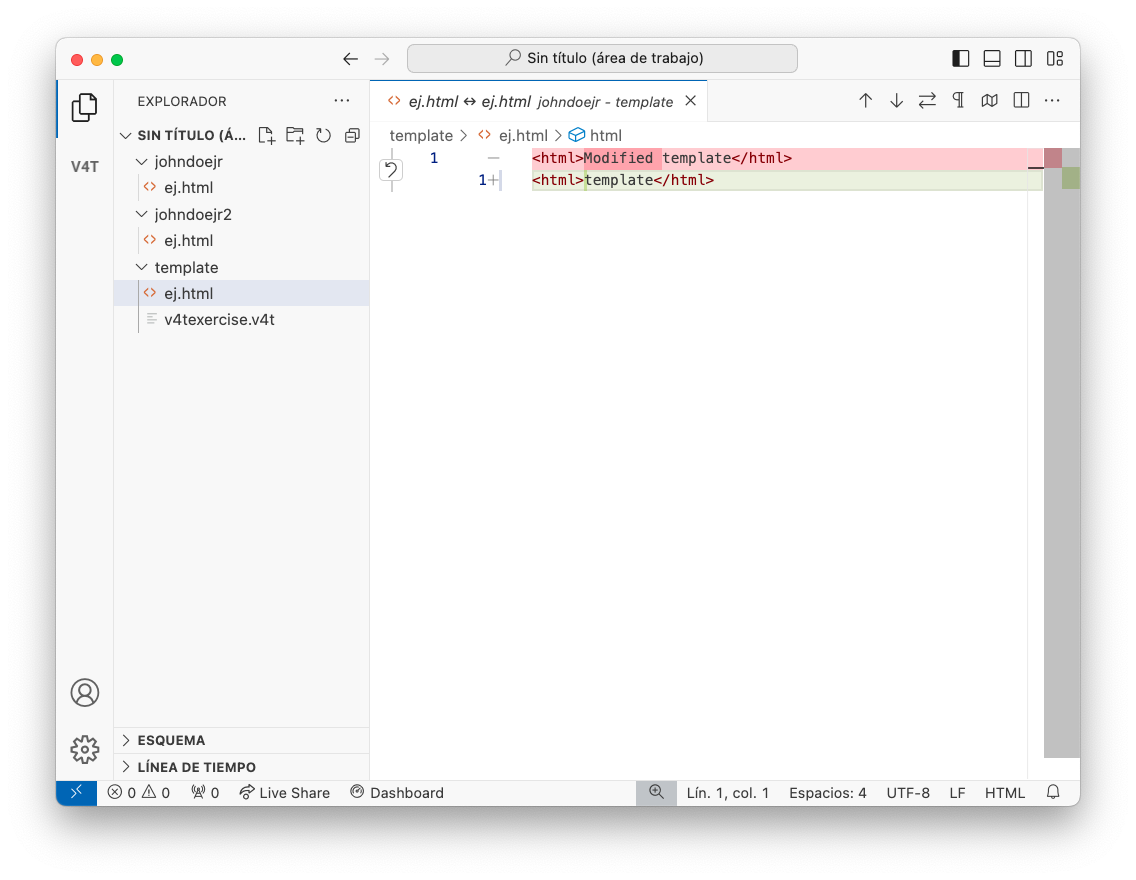
\includegraphics[width=0.825\textwidth]{imagenes/utilizadas/1-introduccion/historia-tfg1-comparacionFicheros.png}
    \caption{Captura de la capacidad para comparación de ficheros en \textit{VSCode4Teaching} en el primer TFG.}
    \label{fig:historiaProyecto1Comparacion}
\end{figure}


El \textbf{segundo} peldaño en la ``escalera'' evolutiva del proyecto \textit{VSCode4Teaching} se produce durante el Trabajo Fin de Grado de Álvaro Justo Rivas Alcobendas \cite{TFG_Alvaro}. Esta contribución potencia la usabilidad de la herramienta, incorporando numerosas características para lograr una experiencia de usuario más completa y que proporcione mejor información sobre todos los procesos de negocio realizados. A este respecto, destaca la incorporación de la actualización en tiempo real del \textit{dashboard} de los docentes y una mejora en su apariencia y funcionalidad, dotándolo de un nuevo estado para los ejercicios ``en progreso'' y de botones para facilitar el acceso a la visualización de los ficheros que componen las propuestas de los estudiantes y sus diferencias respecto a la plantilla original, tal como se refleja en la \referenciaFigura{fig:historiaProyecto2Dashboard}.

\begin{figure}[ht!]
    \centering
    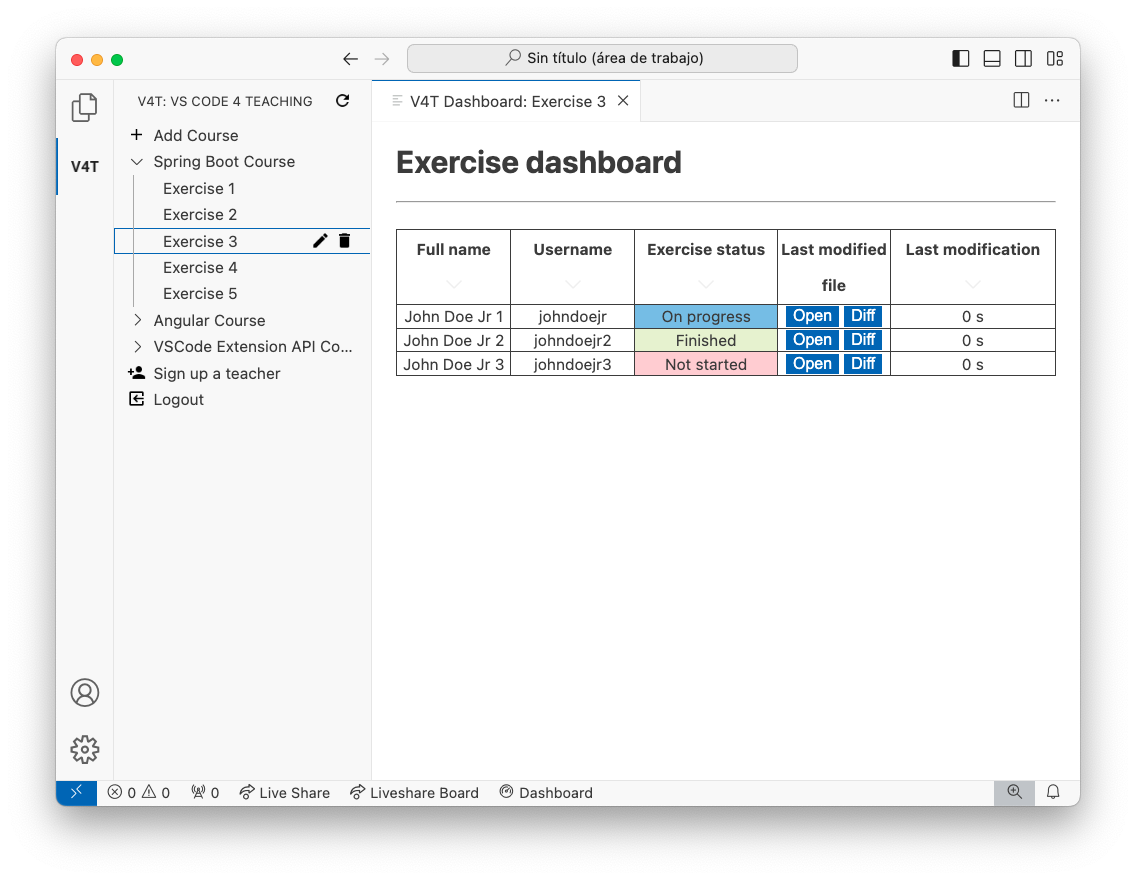
\includegraphics[width=0.825\textwidth]{imagenes/utilizadas/1-introduccion/historia-tfg2-dashboard.png}
    \caption{Captura del \textit{dashboard} para el seguimiento del progreso de los ejercicios en el segundo TFG.}
    \label{fig:historiaProyecto2Dashboard}
\end{figure}

El \textbf{tercer} hito evolutivo del proyecto quedó materializado a través del TFG de Diego Guerrero Carrasco \cite{TFG_Diego1} (autor del presente Trabajo Fin de Grado). Esta iteración añade nuevas funcionalidades, tales como la capacidad para poder añadir a cada ejercicio una propuesta de solución elaborada por el docente, de modo que los estudiantes puedan descargarla cuando el profesor decida hacerla pública y compararla con su propia propuesta de resolución del ejercicio a través de una herramienta gráfica. A esta mejora se suma, además, la capacidad para poder crear múltiples ejercicios a partir de los subdirectorios existentes en una carpeta, la preservación del anonimato de los estudiantes en el sistema de ficheros de la aplicación, de modo que solo el docente pueda relacionar a un alumno con su propuesta de resolución; un nuevo proceso para el alta de docentes basado en un formato de invitaciones entre pares y numerosas mejoras en materia de usabilidad: un menú contextual disponible en los ejercicios y nuevos iconos para mostrar a golpe de vista el progreso en la ejecución de los ejercicios ---tal como refleja la \referenciaFigura{fig:historiaProyecto3GUI}---, una nueva página de ayuda personalizada para cada curso compartido, con información específica del profesor que expide y divulga el código, y un rediseño del \textit{dashboard} para hacerlo más visual e intuitivo ---capturado en la \referenciaFigura{fig:historiaProyecto3Dashboard}---, añadiendo un nuevo gráfico del progreso de los estudiantes y otras métricas numéricas de utilidad sobre el ejercicio. En su faceta técnica, se añade durante esta fase, además, un nuevo componente al proyecto: una aplicación web que sirve como soporte para la implementación de algunas funcionalidades y que actúa de cliente en el modelo cliente-servidor descrito anteriormente.

\begin{figure}[ht!]
    \centering
    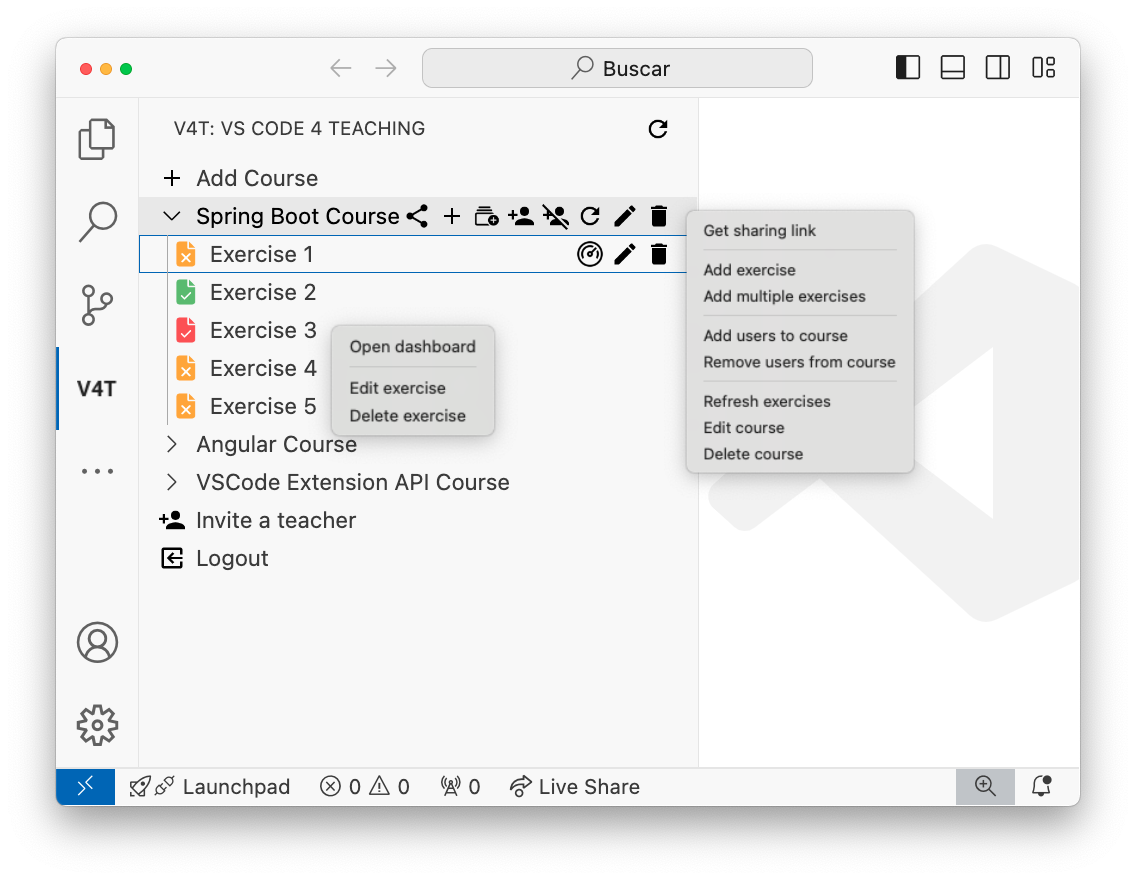
\includegraphics[width=0.825\textwidth]{imagenes/utilizadas/1-introduccion/historia-tfg3-gui.png}
    \caption{Captura de la barra lateral de la extensión con los nuevos iconos y menús contextuales.}
    \label{fig:historiaProyecto3GUI}
\end{figure}

\begin{figure}[ht!]
    \centering
    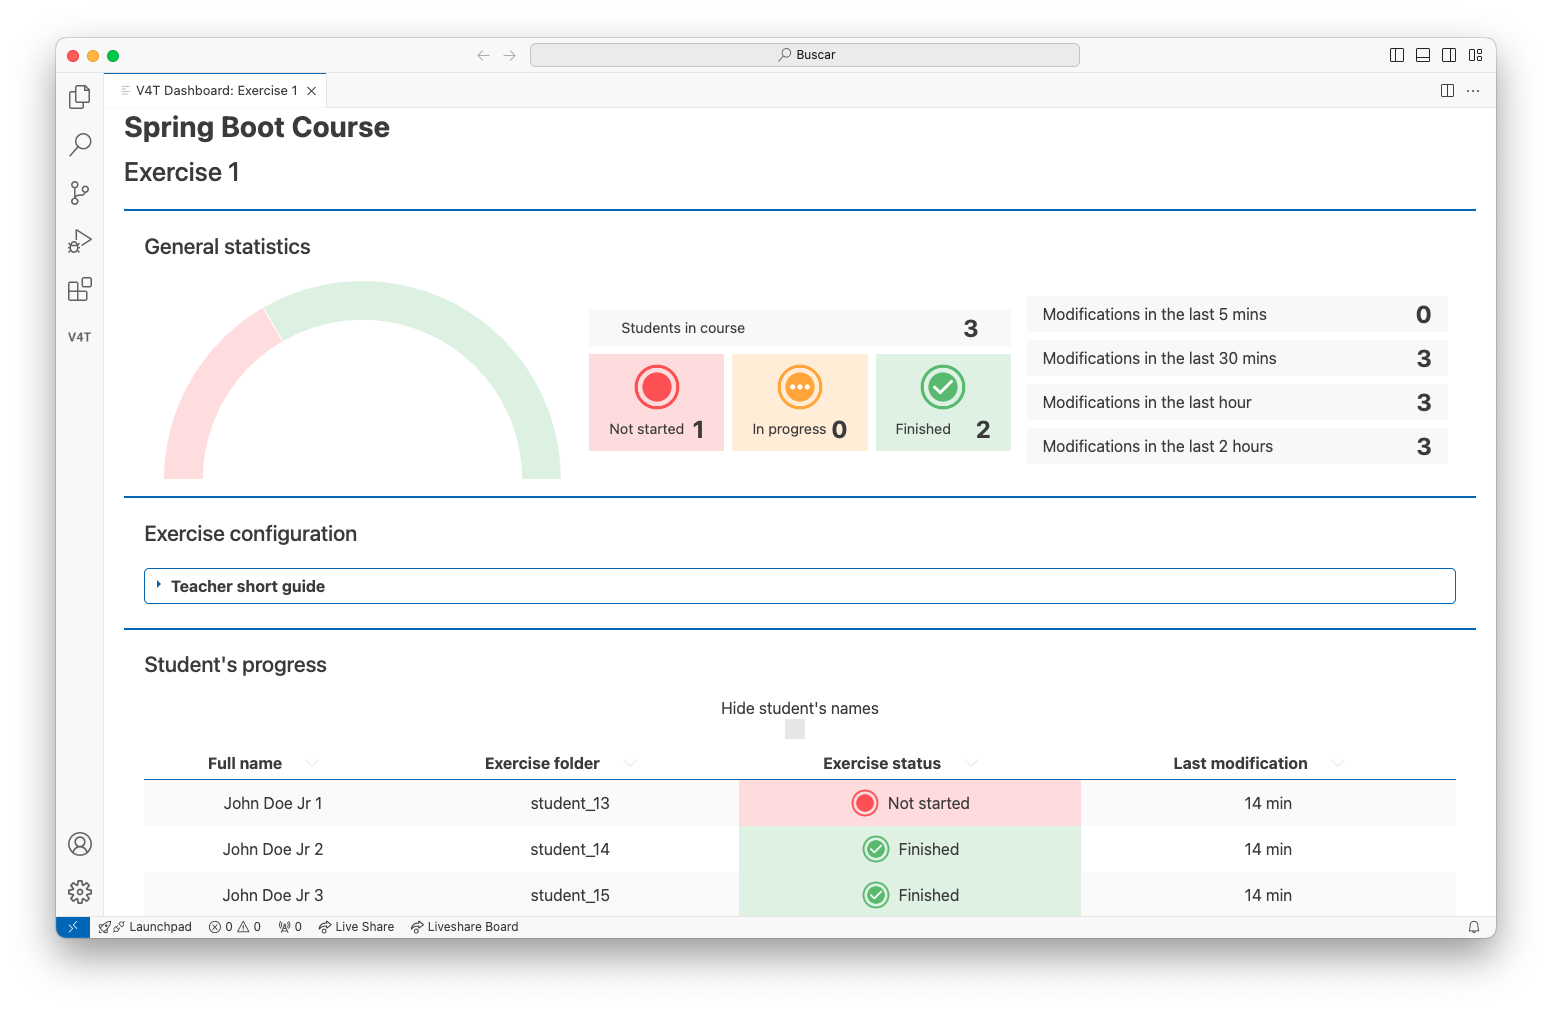
\includegraphics[width=\textwidth]{imagenes/utilizadas/1-introduccion/historia-tfg3-dashboard.png}
    \caption{Captura del \textit{dashboard} para el seguimiento del progreso de los ejercicios en el tercer TFG.}
    \label{fig:historiaProyecto3Dashboard}
\end{figure}

\section{Contexto técnico y motivación}
\label{sec:contxtTecnico}
Una vez planteado el contexto en el que surge la necesidad general del proyecto \textit{VSCode4Teaching} en la \referenciaSeccion{sec:contxtSocial}, y establecido qué es, cómo funciona y cómo se ha construido en la \referenciaSeccion{sec:cronologiaProyecto}, se justifica a continuación la motivación que conduce a realizar el presente Trabajo Fin de Grado.

\textit{VSCode4Teaching} es una aplicación que los usuarios únicamente pueden utilizar a través de un solo IDE\footnote{IDE. Siglas de ``entorno de desarrollo integrado'' (del inglés \textit{Integrated Development Environment}).}: Visual Studio Code.

A este respecto, la \textit{Encuesta sobre el estado de los desarrolladores}, realizada anualmente por JetBrains, recoge en su edición de 2023 \cite{JetBrains_DevState} las respuestas de $26\ 348$ encuestados acerca del uso de distintas tecnologías y herramientas durante el ejercicio de su profesión. De entre ellos, cabe poner el foco en el $19,7\%$ ($5190$) que afirman ser estudiantes de programación. Los datos recogidos para este grupo se incluyen en la \referenciaTabla{tab:usoIDEs}, que refleja las tasas de utilización y preferencia para varios entornos de desarrollo.

\begin{table}
    \caption{Uso de los entornos de desarrollo más populares entre los estudiantes.}
    \label{tab:usoIDEs}
    \centering
    \begin{tabular}{|c|c|c|c|c|}
        \multirow{2}{*}{\textbf{Entorno}} & \multicolumn{2}{c|}{\makecell{\scriptsize Usuarios que lo\\ \textbf{utilizan}}} & \multicolumn{2}{c|}{\makecell{\scriptsize Usuarios que lo\\ \textbf{prefieren}}} \\
        \cline{2-5}
                                          & \textbf{Nº} & \textbf{\%} & \textbf{Nº} & \textbf{\%} \\
        \hline
        Visual Studio Code                & 3512        & 67,67 \%    & 1401        & 26,99 \%    \\
        \hline
        IntelliJ IDEA                     & 2442        & 47,05 \%    & 965         & 18,59 \%    \\
        \hline
        PyCharm                           & 1779        & 34,28 \%    & 424         & 8,17 \%     \\
        \hline
        Visual Studio                     & 1063        & 20,48 \%    & 239         & 4,61 \%     \\
        \hline
        Android Studio                    & 953         & 18,36 \%    & 145         & 2,79 \%     \\
        \hline
        CLion                             & 806         & 15,53 \%    & 164         & 3,16 \%     \\
        \hline
        Vim                               & 745         & 14,35 \%    & 87          & 1,68 \%     \\
        \hline
        WebStorm                          & 725         & 13,97 \%    & 144         & 2,77 \%     \\
        \hline
        Notepad++                         & 595         & 11,46 \%    & 24          & 0,46 \%     \\
        \hline
        \hline
        Total                             & 5190        &             &             &             \\
        \hline
    \end{tabular}
    \\
    {\footnotesize \textbf{Nota:} datos porcentuales respecto al total de estudiantes encuestados.}
\end{table}


Entre los estudiantes destaca Visual Studio Code, siendo un entorno empleado por casi siete de cada diez estudiantes, aunque es el preferido por solo el $27\%$ de este grupo. Sin embargo, la tabla permite constatar que existe un amplio espectro de estudiantes que prefieren utilizar otras opciones, sobresaliendo IntelliJ IDEA y PyCharm, entornos de desarrollo de la empresa JetBrains dedicados a la creación de proyectos sobre las plataformas Java y Python, respectivamente.

Aunque un $67,67\%$ del público objetivo es un porcentaje adecuado, la tasa de estudiantes que afirman preferir Visual Studio Code es sensiblemente inferior, existiendo una gran heterogeneidad en la preferencia por los distintos entornos de desarrollo. De este modo, cabe poner sobre la mesa la posibilidad de ampliar el alcance del proyecto \textit{VSCode4Teaching}, tratando de llegar a la máxima cantidad de usuarios posible. La única alternativa que permitiría alcanzarlo es ofrecer la posibilidad de utilizar la aplicación fuera de Visual Studio Code.

Planteado este escenario, surgen diversas alternativas a ponderar para aumentar el alcance del proyecto. Una de ellas podría ser, por ejemplo, desarrollar una extensión paralela compatible con los entornos de JetBrains, que suman entre todos ellos ---IntelliJ IDEA, PyCharm, CLion y WebStorm en la clasificación anterior--- un $32,69\%$ de preferencia por el estudiantado encuestado. Sin embargo, tal como refleja la documentación de JetBrains al respecto \cite{JetBrains_Plugins}, el conjunto de tecnologías empleado para ello es notablemente diferente del que utiliza la extensión para Visual Studio Code, ya que requieren utilizar Kotlin como lenguaje de programación y Gradle para la gestión de la configuración del \textit{software}, hecho que dificultaría el mantenimiento del proyecto \textit{software} al añadir un componente nuevo que, además, requiere formas de mantenimiento diferentes de los demás y, por otro lado, la cota de público objetivo alcanzado aumenta hasta el $59,69\%$ de usuarios, que es una cifra elevada pero no lo suficientemente como para ejecutar este planteamiento.

Por tanto, la decisión es generar un nuevo cliente distinto de la extensión para Visual Studio Code que se base en una plataforma que sea independiente del IDE que empleen estudiantes o profesores. Generar una aplicación de escritorio conduciría a la misma conclusión que la extrapolada al inicio de este planteamiento, y es que cada usuario puede estar empleando un sistema operativo distinto, hecho que exige la construcción de varias aplicaciones que permitan utilizar \textit{VSCode4Teaching}. Por tanto, de nuevo, la opción de trasladar la funcionalidad a una aplicación de escritorio queda descartada por su complejidad técnica y la dificultad para su mantenimiento.

Con esta motivación y tras el análisis de las opciones disponibles, surge la idea de desarrollar una aplicación web que permita realizar todos los procesos de negocio que \textit{VSCode4Teaching} ya tiene implementados a través de una interfaz. De este modo, los usuarios podrían emplear el entorno de desarrollo y el sistema operativo de su preferencia, dependiendo únicamente del uso de un navegador web actual para garantizar que el proceso más relevante, que es la sincronización bidireccional de ficheros ubicados en el sistema local de los usuarios, puede realizarse correctamente.

\section{Estructura del documento}
\label{sec:estructura}
El presente documento describe detalladamente todos los trabajos realizados sobre el proyecto \textit{VSCode4Teaching} en su cuarto hito evolutivo.

El siguiente apartado (\referenciaCapitulo{cap:objetivos}) establece los objetivos que se buscará satisfacer mediante la realización del Trabajo Fin de Grado.

El tercer punto (\referenciaCapitulo{cap:tecnolHerramMetodo}) recoge el abanico de tecnologías y herramientas empleadas para la ejecución del trabajo, así como la metodología empleada y la organización para su realización.

El apartado cuarto (\referenciaCapitulo{cap:descInformatica}) incluye toda la descripción informática del trabajo ejecutado. Cabe reseñar que la aplicación queda compuesta por tres grandes componentes: el servidor, la extensión para Visual Studio Code y la aplicación web para navegadores, siendo este último el componente sobre el que se implementarán la práctica totalidad de los objetivos y requisitos.

Para finalizar, el capítulo quinto (\referenciaCapitulo{cap:conclusiones}) extrapola conclusiones tras finalizar el desarrollo, analizando la completitud de las necesidades establecidas y analizando trabajos futuros tentativos a realizar en sucesivas iteraciones.

A continuación, una vez finalizado el cuerpo del documento, se introduce la enumeración completa de las referencias bibliográficas a las que aluden las citas introducidas durante el desarrollo del documento.

\noindent\textbf{Nota:} este documento contiene numerosos enlaces e hipervínculos a otras secciones y epígrafes del documento, así como a las referencias bibliográficas, quedando escritos en {\color{RedLink}color rojo}. En su edición electrónica, el lector puede hacer \textit{click} sobre estos enlaces para ser conducido al punto al que referencian.
